\documentclass{beamer}
\usepackage{amsmath}
\usepackage{amssymb}
\usepackage{graphicx}
\begin{document}
\title{Extremal Optimization}
\author{Howon Lee}
\maketitle

\begin{frame}
  \frametitle{What is the question?}
  How can you use extremal dynamics to train some kind of neural net?
\end{frame}

\begin{frame}
  \frametitle{What? What's that?}
  Qualitative model of evolution: Bak-Sneppen model.
  \begin{figure}
    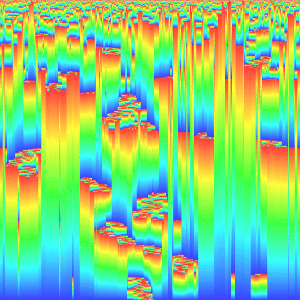
\includegraphics{bak_sneppen}
  \end{figure}

  Rules of Bak-Sneppen model. How does it behave? Criticality. Self-organized criticality.

  Caveats: CR Shalizi, W Tozier, "A Simple Model of the Evolution of Simple Models of Evolution"
\end{frame}

\begin{frame}
  \frametitle{Approaches Taken}
  Bak and Chialvo's model

  More abstract: extremal optimization

  Finally: Using $\tau$-EO on RBM, classification results
\end{frame}

\begin{frame}
  \frametitle{Adaptive Learning by Extremal Dynamics and Negative Feedback}
  How it works, from 20000 feet
  \begin{figure}
    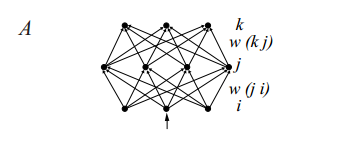
\includegraphics{bak_chialvo_net_topology}
  \end{figure}

  Problems: Conjunctive neurons
  \begin{figure}
    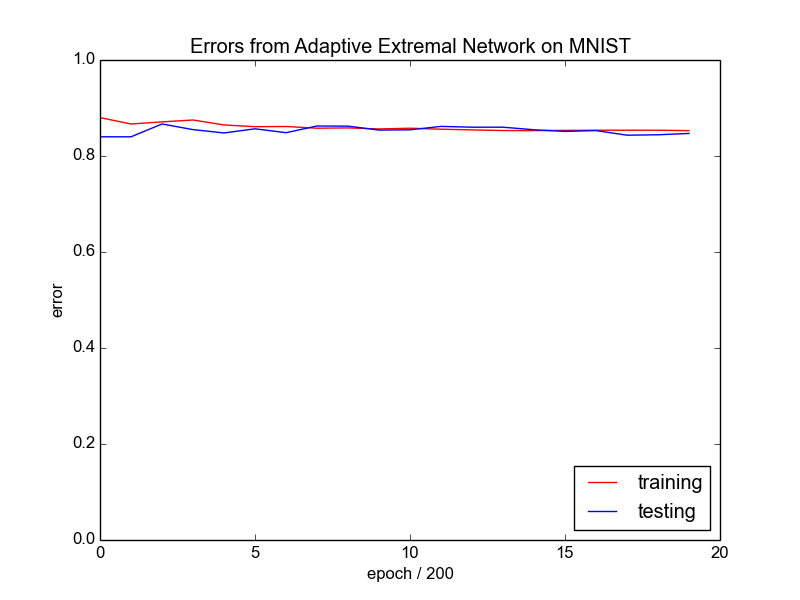
\includegraphics{bak_plot}
  \end{figure}
  
  Comparison to simulated annealing
\end{frame}

\begin{frame}
  \frametitle{More abstractly: EO, $\tau$-EO}
  How it works, from 20000 feet

  Existing results, from Boetticher: TSP, Ising model

  $\tau$-EO
  \begin{figure}
    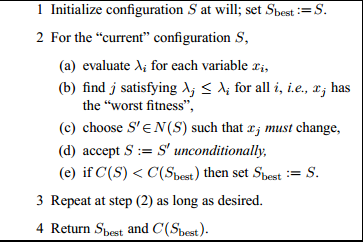
\includegraphics{eo_alg}
  \end{figure}
  %%% steal a chart from Boetticher
\end{frame}

\begin{frame}
  \frametitle{$\tau$-EO on RBM}
  Why not feedforward? BM vs. Ising Model

  Locality: RBM

  \begin{figure}
    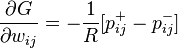
\includegraphics{rbm_eq}
  \end{figure}

  Ising model learning dynamics

  %%% small picture of the low-energy spin glass, then the learning dynamics, and then zoomed in thing showing tau-EO is better
\end{frame}

\begin{frame}
  \frametitle{Task}
  See performance in RBM learning, as simple as possible

  Bit string: metaphor of Hamming cliff in GA

  Actually, this is just a weird coordinate descent
  %%details of approach. specific target phenomenon. model network task setting, architecture, processing and learning algorithm, training environment
  %%% Figuring out applying the abstract EO algorithm to things. Note that the locality of fitness that the model requires is much easier to do in Boltzmann machine, decide to do RBM on those machines.
\end{frame}

\begin{frame}
  \frametitle{Results on RBM}
  \begin{figure}
    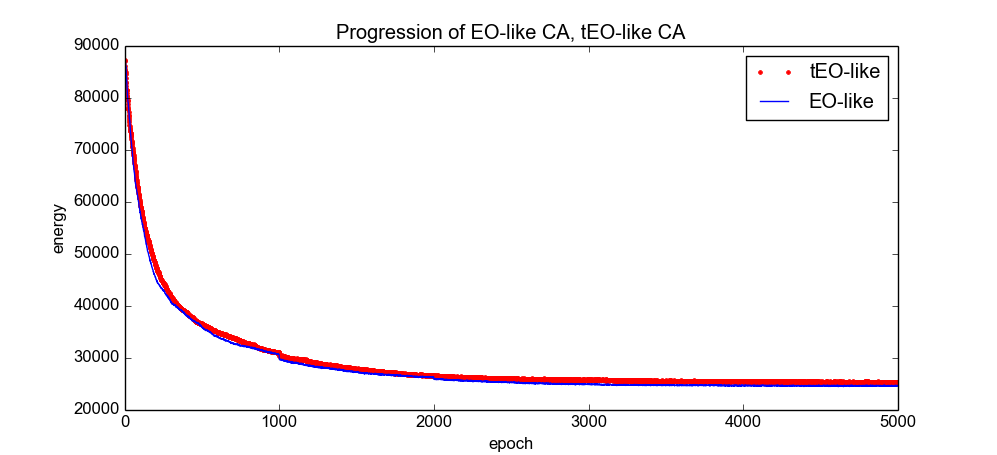
\includegraphics{eo_rbm_unzoomed}
  \end{figure}
  \begin{figure}
    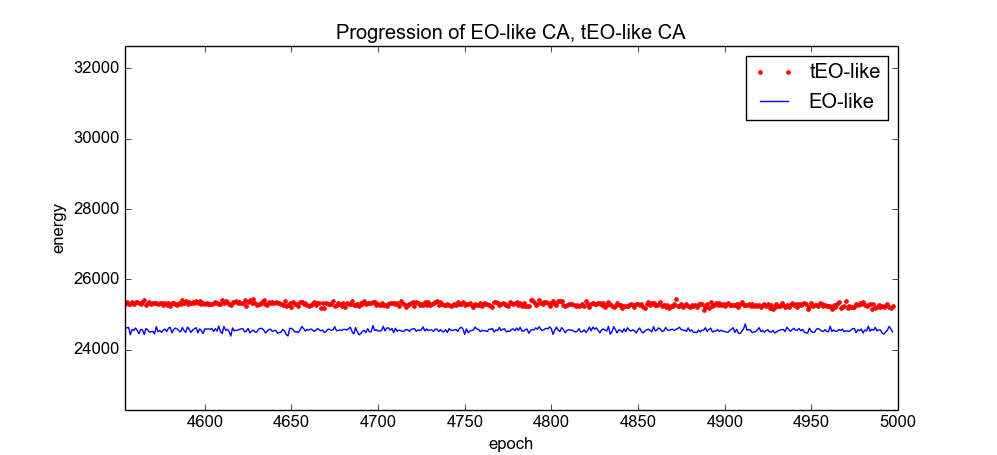
\includegraphics{eo_rbm_zoomed}
  \end{figure}
  %%% look at the weights
\end{frame}

\begin{frame}
  \frametitle{Problems, Issues}
  Make an algorithm that actually differs from CDiv
  Try non-restricted RBM, and learn with regular gradient
  (using EO in place of SA)
\end{frame}

\begin{frame}
  End

  %%% citations
\end{frame}

\end{document}

